% Created by tikzDevice version 0.10.1 on 2018-01-26 10:48:39
% !TEX encoding = UTF-8 Unicode
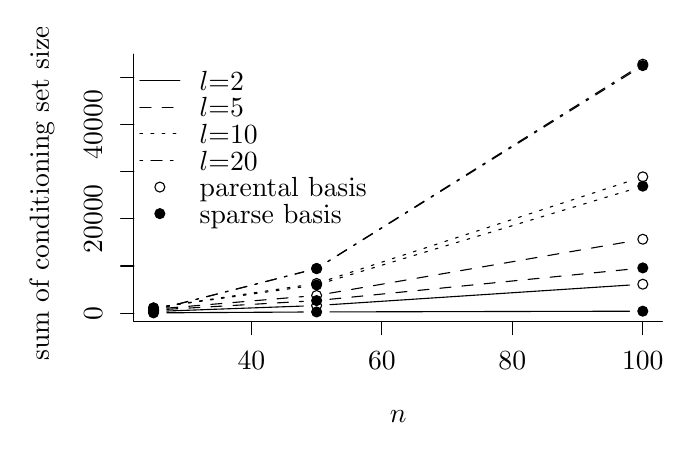
\begin{tikzpicture}[x=1pt,y=1pt]
\definecolor{fillColor}{RGB}{255,255,255}
\path[use as bounding box,fill=fillColor,fill opacity=0.00] (0,0) rectangle (231.26,144.54);
\begin{scope}
\path[clip] ( 38.40, 38.40) rectangle (229.34,134.94);
\definecolor{drawColor}{RGB}{0,0,0}

\path[draw=drawColor,line width= 0.4pt,line join=round,line cap=round] ( 50.27, 42.15) -- ( 99.61, 43.95);

\path[draw=drawColor,line width= 0.4pt,line join=round,line cap=round] (109.20, 44.44) -- (217.48, 51.53);

\path[draw=drawColor,line width= 0.4pt,line join=round,line cap=round] ( 45.47, 41.98) circle (  1.80);

\path[draw=drawColor,line width= 0.4pt,line join=round,line cap=round] (104.41, 44.12) circle (  1.80);

\path[draw=drawColor,line width= 0.4pt,line join=round,line cap=round] (222.27, 51.84) circle (  1.80);
\end{scope}
\begin{scope}
\path[clip] (  0.00,  0.00) rectangle (231.26,144.54);
\definecolor{drawColor}{RGB}{0,0,0}

\path[draw=drawColor,line width= 0.4pt,line join=round,line cap=round] ( 80.83, 38.40) -- (222.27, 38.40);

\path[draw=drawColor,line width= 0.4pt,line join=round,line cap=round] ( 80.83, 38.40) -- ( 80.83, 33.60);

\path[draw=drawColor,line width= 0.4pt,line join=round,line cap=round] (127.98, 38.40) -- (127.98, 33.60);

\path[draw=drawColor,line width= 0.4pt,line join=round,line cap=round] (175.13, 38.40) -- (175.13, 33.60);

\path[draw=drawColor,line width= 0.4pt,line join=round,line cap=round] (222.27, 38.40) -- (222.27, 33.60);

\node[text=drawColor,anchor=base,inner sep=0pt, outer sep=0pt, scale=  1.00] at ( 80.83, 21.12) {40};

\node[text=drawColor,anchor=base,inner sep=0pt, outer sep=0pt, scale=  1.00] at (127.98, 21.12) {60};

\node[text=drawColor,anchor=base,inner sep=0pt, outer sep=0pt, scale=  1.00] at (175.13, 21.12) {80};

\node[text=drawColor,anchor=base,inner sep=0pt, outer sep=0pt, scale=  1.00] at (222.27, 21.12) {100};

\path[draw=drawColor,line width= 0.4pt,line join=round,line cap=round] ( 38.40, 41.38) -- ( 38.40,126.55);

\path[draw=drawColor,line width= 0.4pt,line join=round,line cap=round] ( 38.40, 41.38) -- ( 33.60, 41.38);

\path[draw=drawColor,line width= 0.4pt,line join=round,line cap=round] ( 38.40, 58.41) -- ( 33.60, 58.41);

\path[draw=drawColor,line width= 0.4pt,line join=round,line cap=round] ( 38.40, 75.44) -- ( 33.60, 75.44);

\path[draw=drawColor,line width= 0.4pt,line join=round,line cap=round] ( 38.40, 92.48) -- ( 33.60, 92.48);

\path[draw=drawColor,line width= 0.4pt,line join=round,line cap=round] ( 38.40,109.51) -- ( 33.60,109.51);

\path[draw=drawColor,line width= 0.4pt,line join=round,line cap=round] ( 38.40,126.55) -- ( 33.60,126.55);

\node[text=drawColor,rotate= 90.00,anchor=base,inner sep=0pt, outer sep=0pt, scale=  1.00] at ( 26.88, 41.38) {0};

\node[text=drawColor,rotate= 90.00,anchor=base,inner sep=0pt, outer sep=0pt, scale=  1.00] at ( 26.88, 75.44) {20000};

\node[text=drawColor,rotate= 90.00,anchor=base,inner sep=0pt, outer sep=0pt, scale=  1.00] at ( 26.88,109.51) {40000};

\path[draw=drawColor,line width= 0.4pt,line join=round,line cap=round] ( 38.40,134.94) --
	( 38.40, 38.40) --
	(229.34, 38.40);
\end{scope}
\begin{scope}
\path[clip] (  0.00,  0.00) rectangle (231.26,144.54);
\definecolor{drawColor}{RGB}{0,0,0}

\node[text=drawColor,anchor=base,inner sep=0pt, outer sep=0pt, scale=  1.00] at (133.87,  1.92) {$n$};

\node[text=drawColor,rotate= 90.00,anchor=base,inner sep=0pt, outer sep=0pt, scale=  1.00] at (  7.68, 86.67) {sum of conditioning set sizes};
\end{scope}
\begin{scope}
\path[clip] ( 38.40, 38.40) rectangle (229.34,134.94);
\onlyincolor{\definecolor{drawColor}{RGB}{255,0,0}}
\onlyinblackandwhite{\definecolor{drawColor}{RGB}{0,0,0}}

\path[draw=drawColor,line width= 0.4pt,dash pattern=on 4pt off 4pt ,line join=round,line cap=round] ( 50.25, 43.19) -- ( 99.62, 47.37);

\path[draw=drawColor,line width= 0.4pt,dash pattern=on 4pt off 4pt ,line join=round,line cap=round] (109.14, 48.59) -- (217.54, 67.27);

\path[draw=drawColor,line width= 0.4pt,line join=round,line cap=round] ( 45.47, 42.78) circle (  1.80);

\path[draw=drawColor,line width= 0.4pt,line join=round,line cap=round] (104.41, 47.77) circle (  1.80);

\path[draw=drawColor,line width= 0.4pt,line join=round,line cap=round] (222.27, 68.09) circle (  1.80);
\onlyincolor{\definecolor{drawColor}{RGB}{0,205,0}}

\path[draw=drawColor,line width= 0.4pt,dash pattern=on 1pt off 3pt ,line join=round,line cap=round] ( 50.22, 44.00) -- ( 99.66, 51.40);

\path[draw=drawColor,line width= 0.4pt,dash pattern=on 1pt off 3pt ,line join=round,line cap=round] (108.97, 53.60) -- (217.71, 89.16);

\path[draw=drawColor,line width= 0.4pt,line join=round,line cap=round] ( 45.47, 43.29) circle (  1.80);

\path[draw=drawColor,line width= 0.4pt,line join=round,line cap=round] (104.41, 52.11) circle (  1.80);

\path[draw=drawColor,line width= 0.4pt,line join=round,line cap=round] (222.27, 90.65) circle (  1.80);
\onlyincolor{\definecolor{drawColor}{RGB}{0,0,255}}

\path[draw=drawColor,line width= 0.4pt,dash pattern=on 1pt off 3pt on 4pt off 3pt ,line join=round,line cap=round] ( 50.12, 43.61) -- ( 99.76, 56.34);

\path[draw=drawColor,line width= 0.4pt,dash pattern=on 1pt off 3pt on 4pt off 3pt ,line join=round,line cap=round] (108.47, 60.08) -- (218.20,128.82);

\path[draw=drawColor,line width= 0.4pt,line join=round,line cap=round] ( 45.47, 42.42) circle (  1.80);

\path[draw=drawColor,line width= 0.4pt,line join=round,line cap=round] (104.41, 57.54) circle (  1.80);

\path[draw=drawColor,line width= 0.4pt,line join=round,line cap=round] (222.27,131.36) circle (  1.80);
\definecolor{drawColor}{RGB}{0,0,0}

\path[draw=drawColor,line width= 0.4pt,line join=round,line cap=round] ( 50.27, 41.51) -- ( 99.61, 41.79);

\path[draw=drawColor,line width= 0.4pt,line join=round,line cap=round] (109.21, 41.83) -- (217.47, 42.08);
\definecolor{fillColor}{RGB}{0,0,0}

\path[draw=drawColor,line width= 0.4pt,line join=round,line cap=round,fill=fillColor] ( 45.47, 41.48) circle (  1.80);

\path[draw=drawColor,line width= 0.4pt,line join=round,line cap=round,fill=fillColor] (104.41, 41.82) circle (  1.80);

\path[draw=drawColor,line width= 0.4pt,line join=round,line cap=round,fill=fillColor] (222.27, 42.09) circle (  1.80);
\onlyincolor{\definecolor{drawColor}{RGB}{255,0,0}}

\path[draw=drawColor,line width= 0.4pt,dash pattern=on 4pt off 4pt ,line join=round,line cap=round] ( 50.26, 42.76) -- ( 99.61, 45.64);

\path[draw=drawColor,line width= 0.4pt,dash pattern=on 4pt off 4pt ,line join=round,line cap=round] (109.18, 46.39) -- (217.50, 57.25);
\onlyincolor{\definecolor{fillColor}{RGB}{255,0,0}}

\path[draw=drawColor,line width= 0.4pt,line join=round,line cap=round,fill=fillColor] ( 45.47, 42.48) circle (  1.80);

\path[draw=drawColor,line width= 0.4pt,line join=round,line cap=round,fill=fillColor] (104.41, 45.92) circle (  1.80);

\path[draw=drawColor,line width= 0.4pt,line join=round,line cap=round,fill=fillColor] (222.27, 57.73) circle (  1.80);
\onlyincolor{\definecolor{drawColor}{RGB}{0,205,0}}

\path[draw=drawColor,line width= 0.4pt,dash pattern=on 1pt off 3pt ,line join=round,line cap=round] ( 50.22, 43.93) -- ( 99.65, 50.90);

\path[draw=drawColor,line width= 0.4pt,dash pattern=on 1pt off 3pt ,line join=round,line cap=round] (109.00, 52.96) -- (217.68, 85.88);
\onlyincolor{\definecolor{fillColor}{RGB}{0,205,0}}

\path[draw=drawColor,line width= 0.4pt,line join=round,line cap=round,fill=fillColor] ( 45.47, 43.25) circle (  1.80);

\path[draw=drawColor,line width= 0.4pt,line join=round,line cap=round,fill=fillColor] (104.41, 51.57) circle (  1.80);

\path[draw=drawColor,line width= 0.4pt,line join=round,line cap=round,fill=fillColor] (222.27, 87.27) circle (  1.80);
\onlyincolor{\definecolor{drawColor}{RGB}{0,0,255}}

\path[draw=drawColor,line width= 0.4pt,dash pattern=on 1pt off 3pt on 4pt off 3pt ,line join=round,line cap=round] ( 50.12, 43.60) -- ( 99.75, 56.27);

\path[draw=drawColor,line width= 0.4pt,dash pattern=on 1pt off 3pt on 4pt off 3pt ,line join=round,line cap=round] (108.48, 60.00) -- (218.20,128.29);
\onlyincolor{\definecolor{fillColor}{RGB}{0,0,255}}

\path[draw=drawColor,line width= 0.4pt,line join=round,line cap=round,fill=fillColor] ( 45.47, 42.41) circle (  1.80);

\path[draw=drawColor,line width= 0.4pt,line join=round,line cap=round,fill=fillColor] (104.41, 57.46) circle (  1.80);

\path[draw=drawColor,line width= 0.4pt,line join=round,line cap=round,fill=fillColor] (222.27,130.83) circle (  1.80);
\definecolor{drawColor}{RGB}{0,0,0}

\path[draw=drawColor,line width= 0.4pt,line join=round,line cap=round] ( 40.56,125.34) -- ( 54.96,125.34);
\onlyincolor{\definecolor{drawColor}{RGB}{255,0,0}}

\path[draw=drawColor,line width= 0.4pt,dash pattern=on 4pt off 4pt ,line join=round,line cap=round] ( 40.56,115.74) -- ( 54.96,115.74);
\onlyincolor{\definecolor{drawColor}{RGB}{0,205,0}}

\path[draw=drawColor,line width= 0.4pt,dash pattern=on 1pt off 3pt ,line join=round,line cap=round] ( 40.56,106.14) -- ( 54.96,106.14);
\onlyincolor{\definecolor{drawColor}{RGB}{0,0,255}}

\path[draw=drawColor,line width= 0.4pt,dash pattern=on 1pt off 3pt on 4pt off 3pt ,line join=round,line cap=round] ( 40.56, 96.54) -- ( 54.96, 96.54);
\definecolor{drawColor}{RGB}{0,0,0}

\path[draw=drawColor,line width= 0.4pt,line join=round,line cap=round] ( 47.76, 86.94) circle (  1.80);
\definecolor{fillColor}{RGB}{0,0,0}

\path[draw=drawColor,line width= 0.4pt,line join=round,line cap=round,fill=fillColor] ( 47.76, 77.34) circle (  1.80);

\node[text=drawColor,anchor=base west,inner sep=0pt, outer sep=0pt, scale=  1.00] at ( 62.16,121.90) {$l$=2};

\node[text=drawColor,anchor=base west,inner sep=0pt, outer sep=0pt, scale=  1.00] at ( 62.16,112.30) {$l$=5};

\node[text=drawColor,anchor=base west,inner sep=0pt, outer sep=0pt, scale=  1.00] at ( 62.16,102.70) {$l$=10};

\node[text=drawColor,anchor=base west,inner sep=0pt, outer sep=0pt, scale=  1.00] at ( 62.16, 93.10) {$l$=20};

\node[text=drawColor,anchor=base west,inner sep=0pt, outer sep=0pt, scale=  1.00] at ( 62.16, 83.50) {parental basis};

\node[text=drawColor,anchor=base west,inner sep=0pt, outer sep=0pt, scale=  1.00] at ( 62.16, 73.90) {sparse basis};
\end{scope}
\end{tikzpicture}
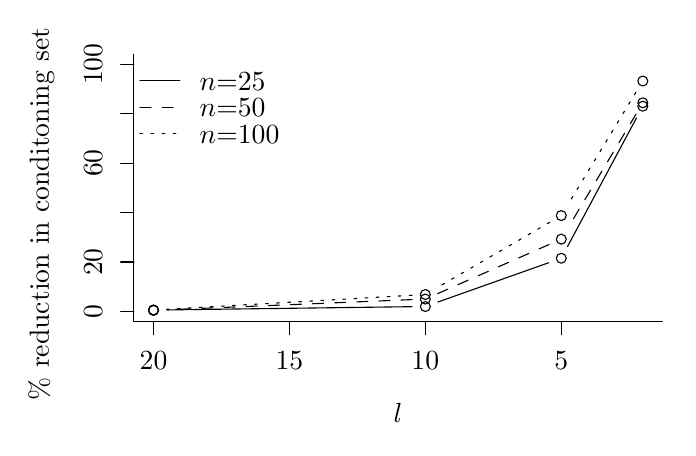
\begin{tikzpicture}[x=1pt,y=1pt]
\definecolor{fillColor}{RGB}{255,255,255}
\path[use as bounding box,fill=fillColor,fill opacity=0.00] (0,0) rectangle (231.26,144.54);
\begin{scope}
\path[clip] ( 38.40, 38.40) rectangle (229.34,134.94);
\definecolor{drawColor}{RGB}{0,0,0}

\path[draw=drawColor,line width= 0.4pt,line join=round,line cap=round] (220.00,111.93) -- (195.07, 65.45);

\path[draw=drawColor,line width= 0.4pt,line join=round,line cap=round] (188.28, 59.61) -- (148.22, 45.39);

\path[draw=drawColor,line width= 0.4pt,line join=round,line cap=round] (138.89, 43.72) -- ( 50.27, 42.55);

\path[draw=drawColor,line width= 0.4pt,line join=round,line cap=round] (222.27,116.16) circle (  1.80);

\path[draw=drawColor,line width= 0.4pt,line join=round,line cap=round] (192.81, 61.22) circle (  1.80);

\path[draw=drawColor,line width= 0.4pt,line join=round,line cap=round] (143.69, 43.78) circle (  1.80);

\path[draw=drawColor,line width= 0.4pt,line join=round,line cap=round] ( 45.47, 42.49) circle (  1.80);
\end{scope}
\begin{scope}
\path[clip] (  0.00,  0.00) rectangle (231.26,144.54);
\definecolor{drawColor}{RGB}{0,0,0}

\path[draw=drawColor,line width= 0.4pt,line join=round,line cap=round] (192.81, 38.40) -- ( 45.47, 38.40);

\path[draw=drawColor,line width= 0.4pt,line join=round,line cap=round] (192.81, 38.40) -- (192.81, 33.60);

\path[draw=drawColor,line width= 0.4pt,line join=round,line cap=round] (143.69, 38.40) -- (143.69, 33.60);

\path[draw=drawColor,line width= 0.4pt,line join=round,line cap=round] ( 94.58, 38.40) -- ( 94.58, 33.60);

\path[draw=drawColor,line width= 0.4pt,line join=round,line cap=round] ( 45.47, 38.40) -- ( 45.47, 33.60);

\node[text=drawColor,anchor=base,inner sep=0pt, outer sep=0pt, scale=  1.00] at ( 45.47, 21.12) {20};

\node[text=drawColor,anchor=base,inner sep=0pt, outer sep=0pt, scale=  1.00] at ( 94.58, 21.12) {15};

\node[text=drawColor,anchor=base,inner sep=0pt, outer sep=0pt, scale=  1.00] at (143.69, 21.12) {10};

\node[text=drawColor,anchor=base,inner sep=0pt, outer sep=0pt, scale=  1.00] at (192.81, 21.12) {5};

\path[draw=drawColor,line width= 0.4pt,line join=round,line cap=round] ( 38.40, 41.98) -- ( 38.40,131.36);

\path[draw=drawColor,line width= 0.4pt,line join=round,line cap=round] ( 38.40, 41.98) -- ( 33.60, 41.98);

\path[draw=drawColor,line width= 0.4pt,line join=round,line cap=round] ( 38.40, 59.85) -- ( 33.60, 59.85);

\path[draw=drawColor,line width= 0.4pt,line join=round,line cap=round] ( 38.40, 77.73) -- ( 33.60, 77.73);

\path[draw=drawColor,line width= 0.4pt,line join=round,line cap=round] ( 38.40, 95.61) -- ( 33.60, 95.61);

\path[draw=drawColor,line width= 0.4pt,line join=round,line cap=round] ( 38.40,113.49) -- ( 33.60,113.49);

\path[draw=drawColor,line width= 0.4pt,line join=round,line cap=round] ( 38.40,131.36) -- ( 33.60,131.36);

\node[text=drawColor,rotate= 90.00,anchor=base,inner sep=0pt, outer sep=0pt, scale=  1.00] at ( 26.88, 41.98) {0};

\node[text=drawColor,rotate= 90.00,anchor=base,inner sep=0pt, outer sep=0pt, scale=  1.00] at ( 26.88, 59.85) {20};

\node[text=drawColor,rotate= 90.00,anchor=base,inner sep=0pt, outer sep=0pt, scale=  1.00] at ( 26.88, 95.61) {60};

\node[text=drawColor,rotate= 90.00,anchor=base,inner sep=0pt, outer sep=0pt, scale=  1.00] at ( 26.88,131.36) {100};

\path[draw=drawColor,line width= 0.4pt,line join=round,line cap=round] ( 38.40,134.94) --
	( 38.40, 38.40) --
	(229.34, 38.40);
\end{scope}
\begin{scope}
\path[clip] (  0.00,  0.00) rectangle (231.26,144.54);
\definecolor{drawColor}{RGB}{0,0,0}

\node[text=drawColor,anchor=base,inner sep=0pt, outer sep=0pt, scale=  1.00] at (133.87,  1.92) {$l$};

\node[text=drawColor,rotate= 90.00,anchor=base,inner sep=0pt, outer sep=0pt, scale=  1.00] at (  7.68, 86.67) {\% reduction in conditoning set size};
\end{scope}
\begin{scope}
\path[clip] ( 38.40, 38.40) rectangle (229.34,134.94);
\onlyincolor{\definecolor{drawColor}{RGB}{255,0,0}}
\onlyinblackandwhite{\definecolor{drawColor}{RGB}{0,0,0}}

\path[draw=drawColor,line width= 0.4pt,dash pattern=on 4pt off 4pt ,line join=round,line cap=round] (219.81,113.27) -- (195.27, 72.24);

\path[draw=drawColor,line width= 0.4pt,dash pattern=on 4pt off 4pt ,line join=round,line cap=round] (188.41, 66.18) -- (148.09, 48.41);

\path[draw=drawColor,line width= 0.4pt,dash pattern=on 4pt off 4pt ,line join=round,line cap=round] (138.90, 46.28) -- ( 50.27, 42.59);

\path[draw=drawColor,line width= 0.4pt,line join=round,line cap=round] (222.27,117.39) circle (  1.80);

\path[draw=drawColor,line width= 0.4pt,line join=round,line cap=round] (192.81, 68.12) circle (  1.80);

\path[draw=drawColor,line width= 0.4pt,line join=round,line cap=round] (143.69, 46.48) circle (  1.80);

\path[draw=drawColor,line width= 0.4pt,line join=round,line cap=round] ( 45.47, 42.39) circle (  1.80);
\onlyincolor{\definecolor{drawColor}{RGB}{0,205,0}}

\path[draw=drawColor,line width= 0.4pt,dash pattern=on 1pt off 3pt ,line join=round,line cap=round] (219.78,121.17) -- (195.29, 80.75);

\path[draw=drawColor,line width= 0.4pt,dash pattern=on 1pt off 3pt ,line join=round,line cap=round] (188.65, 74.23) -- (147.84, 50.52);

\path[draw=drawColor,line width= 0.4pt,dash pattern=on 1pt off 3pt ,line join=round,line cap=round] (138.90, 47.84) -- ( 50.26, 42.78);

\path[draw=drawColor,line width= 0.4pt,line join=round,line cap=round] (222.27,125.27) circle (  1.80);

\path[draw=drawColor,line width= 0.4pt,line join=round,line cap=round] (192.81, 76.64) circle (  1.80);

\path[draw=drawColor,line width= 0.4pt,line join=round,line cap=round] (143.69, 48.11) circle (  1.80);

\path[draw=drawColor,line width= 0.4pt,line join=round,line cap=round] ( 45.47, 42.51) circle (  1.80);
\definecolor{drawColor}{RGB}{0,0,0}

\path[draw=drawColor,line width= 0.4pt,line join=round,line cap=round] ( 40.56,125.34) -- ( 54.96,125.34);
\onlyincolor{\definecolor{drawColor}{RGB}{255,0,0}}

\path[draw=drawColor,line width= 0.4pt,dash pattern=on 4pt off 4pt ,line join=round,line cap=round] ( 40.56,115.74) -- ( 54.96,115.74);
\onlyincolor{\definecolor{drawColor}{RGB}{0,205,0}}

\path[draw=drawColor,line width= 0.4pt,dash pattern=on 1pt off 3pt ,line join=round,line cap=round] ( 40.56,106.14) -- ( 54.96,106.14);
\definecolor{drawColor}{RGB}{0,0,0}

\node[text=drawColor,anchor=base west,inner sep=0pt, outer sep=0pt, scale=  1.00] at ( 62.16,121.90) {$n$=25};

\node[text=drawColor,anchor=base west,inner sep=0pt, outer sep=0pt, scale=  1.00] at ( 62.16,112.30) {$n$=50};

\node[text=drawColor,anchor=base west,inner sep=0pt, outer sep=0pt, scale=  1.00] at ( 62.16,102.70) {$n$=100};
\end{scope}
\end{tikzpicture}
